\chapter{Project Plan}
\label{chap:project-plan}

\section{Deliverables}
\label{sec:deliverables}
\vspace{-3mm}
\textbf{\underline{Final UI design \& brand guidelines}}
\par
\textbf{Due date:} 13/12/21
\par
\vspace{-3mm}
\textbf{Description:} The finalized branding and user interface designs for all major screens of the application.
These will be used during development for reference and to create reusable components (``widgets'' in Flutter) for consistency across
the application. The branding is also important for further marketing of \textit{the product} in future.
\par
\vspace{-3mm}
\textbf{Success criterion:} Easy-to-follow guidance for developers. No further questions
should be asked from developers as the guidance should be comprehensive enough for complete development.
\par

\textbf{\underline{Reusable UI Components (``Widgets'') - and test cases}}
\par
\textbf{Due date:} 24/12/21
\par
\vspace{-3mm}
\textbf{Description:} Custom Flutter widgets that complete the design system put forward in the guidelines. Any developer will use
these widgets to produce consistent frontend code. Custom test cases must be written to verify these function as normal (buttons etc.).
\par
\vspace{-3mm}
\textbf{Success criterion:} No errors should be found when using custom widgets in place of default widgets during early stage development. All Flutter widget tests should pass.
\par
\pagebreak

\textbf{\underline{Minimum Viable Product}}
\par
\textbf{Due date:} 31/01/22
\par
\vspace{-3mm}
\textbf{Description:} A fully functional and ready-to-test application that features all the core features. The bare minimum product
that could satisfy the aims we set in \cref{sec:intro_overview}. The overall
efficiency and elegance of the UI is not as crucial as the functionality at this stage.
\par
\vspace{-3mm}
\textbf{Success criterion:} Any stakeholder or external user could comfortably agree that the aims have been met when
using the app. It should be demonstrable.
\par

\textbf{\underline{Complete Test Suite(s)}}
\par
\textbf{Due date:} 14/02/22
\par
\vspace{-3mm}
\textbf{Description:} A comprehensive collection of tests for the Flutter application (and ideally for the Express API).
This should be composed of existing widget tests, unit tests for specific functionality and
integration tests for when the system is ready to be thoroughly tested. The ``system under test'' must be clearly defined where applicable.
\par
\vspace{-3mm}
\textbf{Success criterion:} Test coverage must cover all requirements set in \cref{sec:requirements} as well as architectural data paths
visualised in \cref{fig:architecture-diagram} (thorough structural coverage). Tests must satisfy that the features desired (\cref{sec:features}) are
tested and function as expected.
\par

\textbf{\underline{MVP Test Results}}
\par
\textbf{Due date:} 21/02/22
\par
\vspace{-3mm}
\textbf{Description:} Results and actions to take following the application of the test suite to the MVP.
\par
\vspace{-3mm}
\textbf{Success criterion:} All tests have actionable results - pass/fail must be accompanied by a relevant message describing
the outcome(s) and next steps (if any).
\par

\textbf{\underline{Project completion \& presentation created}}
\par
\textbf{Due date:} 15/03/22
\par
\vspace{-3mm}
\textbf{Description:} All relevant testing changes made. A presentation document should accompany the final product ready for demonstration
to stakeholders during the project fair. Usability and efficiency are not of utmost importance but should be prioritized.
\par
\vspace{-3mm}
\textbf{Success criterion:} A functional application that satisfies all aims and passes all test cases.
\par
\pagebreak

\textbf{\underline{Dissertation}}
\par
\textbf{Due date:} 03/05/22
\par
\vspace{-3mm}
\textbf{Description:} A documentation of the progress and development of the project through to completion. This forms a large portion of the basis
for grading of the project and the deadline is final.
\par
\vspace{-3mm}
\textbf{Success criterion:} A thoroughly well written document that describes the development process as well as lessons learnt from the project.

\vspace{-5mm}
\section{Project schedule}
\begin{figure}[H]
    \noindent\makebox[\textwidth]{
        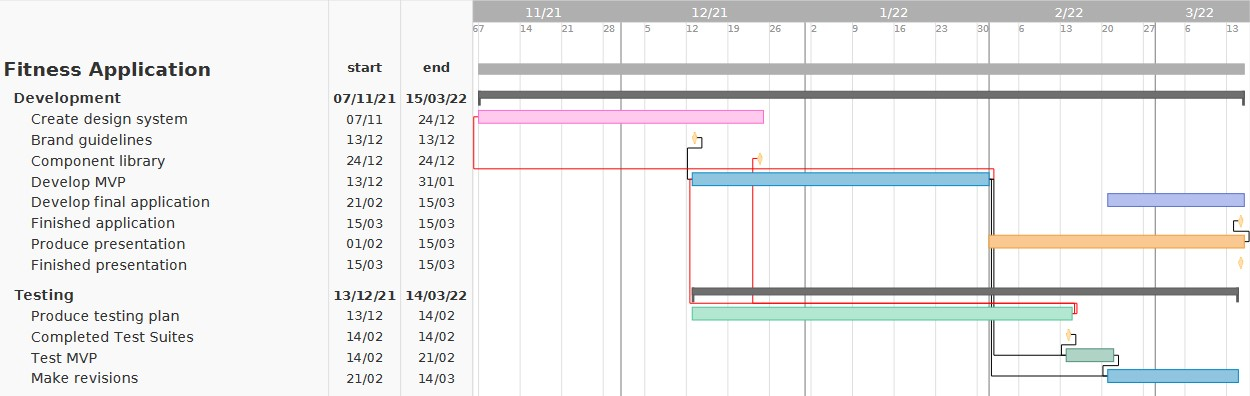
\includegraphics[width=1.2\textwidth]{graphics/gantt-chart.jpg}}
    \caption{An overview Gantt chart, clearly outlining milestones and phases.}
    \label{fig:gantt}
\end{figure}
\vspace{-5mm}
The project has begun already as seen in \cref{chap:preliminary-work}, however
we are using 07/11/21 as an acting ``start date''. We expect the project to be completed by
15/03/22. There is some float as seen in the above Gantt chart (\cref{fig:gantt});
mainly focused on the end of the MVP development phase and testing. Having some leverage
here means we can adjust our schedule dependent on the volume of changes that need to be implemented.
\vspace{-5mm}
\subsection{Limitations}
\vspace{-3mm}
Our main limitations are time and scope. As established in \cref{chap:intro},
the project is different and has a more narrow scope than \textit{the product}.
Spending too much time refining code and not focusing on implementation of complex features will mean
the grade achieved for the project is low(er) due to us not meeting the aims we have outlined in this document.
Time is a factor in this problem as it must be used wisely and we must aim to stick to the project schedule in order
to complete the core functionality (and by extension, the project) on time. These risks are assessed later (\cref{sec:risk}).
\pagebreak

\section{Software development strategy}
We intend on following a ``Feature-driven development'' (FDD) model - an iterative and incremental software development
process. The rationale here is that the bulk of our success criterion rely on the features (functionality) of our
application. Focusing on establishing features first will mean we are more likely to
fulfill our aims - albeit at the expense of thorough testing during development.
\subsection{Choice of model}
As mentioned prior, FDD is an iterative process; it comfortably falls under the ``Agile'' methodology umbrella.
Agile models like FDD are more adaptable and mean that decisions can be made following short sprints of code without
drastic further impact on our project schedule and lifecycle. Whilst it's true that we run the risk of
making brash decisions, this can be mitigated by having regular reviews (stand-ups) and
in our case, sanity checks and meetings with the project supervisor(s) and other stakeholders.
\par
The decision to follow an Agile approach specifically is due to the tight deadlines and
unclear final product. By reviewing development frequently and focusing on developing features of the application, we are
less likely to encounter scope creep and more likely to satisfy the success criteria we have established.
For the sake of argument, let's suppose we followed a traditional SDLC model (think Waterfall, Spiral, V-Shape).
We'd have to spend significant time outlining clear phases of our lifecycle and focusing on said phases in sequence (with most models).
This would mean less time is left for development before March and given the unfamiliarity with
the proposed technology stack this would dramatically increase the risk of not completing the application (or worse the MVP).
Adapting to roadblocks would also require pauses in development and alteration of our
predetermined phases (such as testing). This (again) increases our risk of failure.
\par
Ultimately, whilst traditional SDLC models are sufficient for large-scale well-documented projects with
comprehensive feasibility reports and cost-benefit analyses - it is not ideal
when we are completing a project single-handedly under strong time constraints.
Deadlines are thoroughly fixed and without sacrificing performance
in the degree it would be difficult to follow said models well.
\pagebreak

\subsection{Testing lifecycle}
We'll be using aspects of ``Behaviour-driven Development'' (BDD) which is an extension of
``Test-driven Development''. Our use of BDD is only relevant to the testing approach we'll be following.
BDD testing uses human-readable descriptions of user requirements (similar to those in \cref{sec:requirements}) as the
basis for software tests. The process involves defining entities, events and outputs with given names before using
the names to encode system tests. Each test is based on a user story written using the aforementioned vocabulary.
For example:
\vspace{-5mm}
\begin{verbatim}
    Story: User can create a new exercise

    As an end user,
    In order to add new exercises
    I add video sources to a text description.

    On the create workout page,
    I press create new exercise,
    describe the exercise and add a video source
    before selecting "ok".
    Then my new exercise should appear
    as an option when creating a workout.
\end{verbatim}
\vspace{-5mm}
These tests are then translated into a programming language (in our case Dart code for Flutter)
to produce unit tests. We'll be following a black-box testing method, meaning
we aren't concerned with the internal workings behind the tests; we are only 
testing the functionality and not the implementation. This decouples
our tests from our code and means there is less to refactor if/when our code
is revised.
\par
For this project it's not likely we add much automation to our testing beyond where it is natural
such as widgets and other simple unit tests. Because deployment is outside of the scope of the project,
there is no significant reason to form a strong CI/CD pipeline.
\par
Our test results will be documented in a test summary report. This works similarly to this 
project proposal report and means that any stakeholder can read a brief report on how and what results were
found following our test phase. Following revisions, we will repeat the testing and add tests
if needed for future enhancements.

\section{Risk management plan}
\label{sec:risk}
We'll be using a risk register to document and describe risks below - this will form the single source where
risks can be documented and added/altered (based on changes in resources).
\par
\textbf{Risk description:} A description of the risk we're encountering.\\
\textbf{Probability of occurrence:} How likely the risk is to occur (using percentage).\\
\textbf{Severity:} The intensity of the risk on a 1-4 scale - low, medium, high, extremely high.\\
\textbf{Status:} View of the risk - potential, monitoring, occurring, or eliminated.\\
\textbf{Loss size (days):} Measuring the negative impact the occurrence of the risk would have.\\

\subsection{Risk analysis}
\textbf{Risk description:} File changes lost.\\
\vspace{-2mm}
\textbf{Probability of occurrence:} 5\%\\
\vspace{-2mm}
\textbf{Severity:} 1\\
\vspace{-2mm}
\textbf{Status:} potential\\
\vspace{-2mm}
\textbf{Loss size (days):} 1\\
\textbf{Mitigation strategy:} \cref{risk:mitigation-files}\\

\par

\hrulefill

\textbf{Risk description:} Behind on project schedule.\\
\vspace{-2mm}
\textbf{Probability of occurrence:} 50\%\\
\vspace{-2mm}
\textbf{Severity:} 2\\
\vspace{-2mm}
\textbf{Status:} monitoring\\
\vspace{-2mm}
\textbf{Loss size (days):} 7\\
\textbf{Mitigation strategy:} \cref{risk:mitigation-timeline}\\

\par

\hrulefill

\textbf{Risk description:} Scope creep.\\
\vspace{-2mm}
\textbf{Probability of occurrence:} 10\%\\
\vspace{-2mm}
\textbf{Severity:} 2\\
\vspace{-2mm}
\textbf{Status:} monitoring\\
\vspace{-2mm}
\textbf{Loss size (days):} 3\\
\textbf{Mitigation strategy:} \cref{risk:mitigation-scope}\\

\par

\pagebreak


\textbf{Risk description:} Contraction of COVID-19 or other illness.\\
\vspace{-2mm}
\textbf{Probability of occurrence:} 5\%\\
\vspace{-2mm}
\textbf{Severity:} 3\\
\vspace{-2mm}
\textbf{Status:} potential\\
\vspace{-2mm}
\textbf{Loss size (days):} 10\\
\vspace{-1mm}
\textbf{Mitigation strategy:} \cref{risk:mitigation-covid}\\


\hrulefill

\textbf{Risk description:} Travel delays without access to codebase.\\
\vspace{-2mm}
\textbf{Probability of occurrence:} 30\%\\
\vspace{-2mm}
\textbf{Severity:} 4\\
\vspace{-2mm}
\textbf{Status:} potential\\
\vspace{-2mm}
\textbf{Loss size (days):} 3\\
\textbf{Mitigation strategy:} \cref{risk:mitigation-travel}\\
\par

\hrulefill

\textbf{Risk description:} Technical knowledge roadblocks\\
\vspace{-2mm}
\textbf{Probability of occurrence:} 90\%\\
\vspace{-2mm}
\textbf{Severity:} 3\\
\vspace{-2mm}
\textbf{Status:} monitoring\\
\vspace{-2mm}
\textbf{Loss size (days):} 14\\
\textbf{Mitigation strategy:} \cref{risk:mitigation-roadblocks}\\
\par

\subsection{Risk mitigation}
\subsubsection{File changes lost:}
\label{risk:mitigation-files}
\vspace{-2mm}
This risk will be mitigated if encountered by using git version control and GitHub remote repositories.
The developer(s) will commit code periodically during development of features
and at minimum 1x per day (at COB \footnote{Close of business = 5pm}).

\subsubsection{Behind on project schedule:}
\label{risk:mitigation-timeline}
\vspace{-2mm}
The risk here is low given the float we have in our project schedule.
If this occurs then the bottleneck will be identified before considering
which other processes can continue in tandem with finding a solution. This risk 
is prevalent during all stages of the project and avoidance is better than mitigation.
Mitigation strategies are largely dependent on identifying the bottleneck delaying the project.
In general this will involve trading personal self-study for crisis resolution - the worst case is 1 complete week is lost
getting back on schedule.

\subsubsection{Scope creep:}
\label{risk:mitigation-scope}
\vspace{-2mm}
To avoid scope creep in the first instance, the project requirements will be tracked on a Kanban-style board during
feature-driven development. To mitigate any scope creep I will schedule regular sanity checks with my supervisor and
make use of ``rubber duck debugging'' to consciously hear what is being worked on.
Code reviews will take place via GitHub pull requests and the labelling of features
as ``enhancements'' will be used to mitigate the creeping in of new functionality and aims.

\subsubsection{Contraction of COVID-19 or other illness:}
\label{risk:mitigation-covid}
\vspace{-2mm}
I will actively avoid large gatherings and wear a mask where possible. I have received my 2nd vaccine and will
stay updated on the status of a booster vaccine if it provides sufficient efficacy
for avoiding covid-19. To mitigate the risk once contracted I will rest
and self isolate until recovered. This risk is one of the most difficult to mitigate as 
it involves personal health - without which I cannot actively work on the project.

\subsubsection{Travel delays without access to codebase:}
\label{risk:mitigation-travel}
\vspace{-2mm}
Being delayed during flights and trains without stable internet access is more than likely given
the global situation. To mitigate this risk I will use GitHub and carry a ``MiFi'' 4G router when travelling.
This means access to the code should be possible with just my GitHub credentials. In extreme circumstances,
I will clone the repository and work locally on a temporary machine before reaching home to comfortably push changes back.
I don't expect delays surpassing 3 days and there has been sufficient time allocated in the project schedule to 
limit the effects of any delays.

\subsubsection{Technical knowledge roadblocks:}
\label{risk:mitigation-roadblocks}
\vspace{-2mm}
This risk is inevitable given the project scope and development experience.
To mitigate this risk I will make extensive use of the Flutter forum(s) including
StackOverflow. This risk could mean the failure of the project - in which case
mitigation would involve drastically reframing the projects aims to be more achievable and avoid
the roadblock being encountered.

